\section*{Task 6}

\subsection*{Task statement}

Drive your robot model between 2 consequent points. (Solve polynomial)

\subsection*{Solution}

Here I used quintic polynomial in the following form:

$$q(t) = a_5 t^5 + a_4 t^4 + a_3 t^3 + a_2 t^2 + a_1 t_1 + a_0$$

To find coefficients of the polynomial, I solved the following linear system of equations:

$$
\begin{pmatrix}
    t_0^5 & t_0^4 & t_0^3 & t_0^2 & t_0 & 1 \\
    t_f^5 & t_f^4 & t_f^3 & t_f^2 & t_f & 1 \\
    5t_0^4 & 4t_0^3 & 3t_0^2 & 2t_0 & 1 & 0 \\
    5t_f^4 & 4t_f^3 & 3t_f^2 & 2t_f & 1 & 0 \\
    20t_0^3 & 12t_0^2 & 6t_0 & 2 & 0 & 0 \\
    20t_f^3 & 12t_f^2 & 6t_f & 2 & 0 & 0 \\
\end{pmatrix}
\begin{pmatrix}
    a_5 \\ a_4 \\ a_3 \\ a_2 \\ a_1 \\ a_0
\end{pmatrix}
=
\begin{pmatrix}
    q_0 \\
    q_f \\
    \dot q_0 \\
    \dot q_f \\
    \ddot q_0 \\
    \ddot q_f
\end{pmatrix}
$$

Then we can calculate positions for each moment of time:

$$q(t) = \begin{pmatrix}
    t_0^5 & t_0^4 & t_0^3 & t_0^2 & t_0 & 1
\end{pmatrix}
\begin{pmatrix}
    a_5 \\ a_4 \\ a_3 \\ a_2 \\ a_1 \\ a_0
\end{pmatrix}
$$

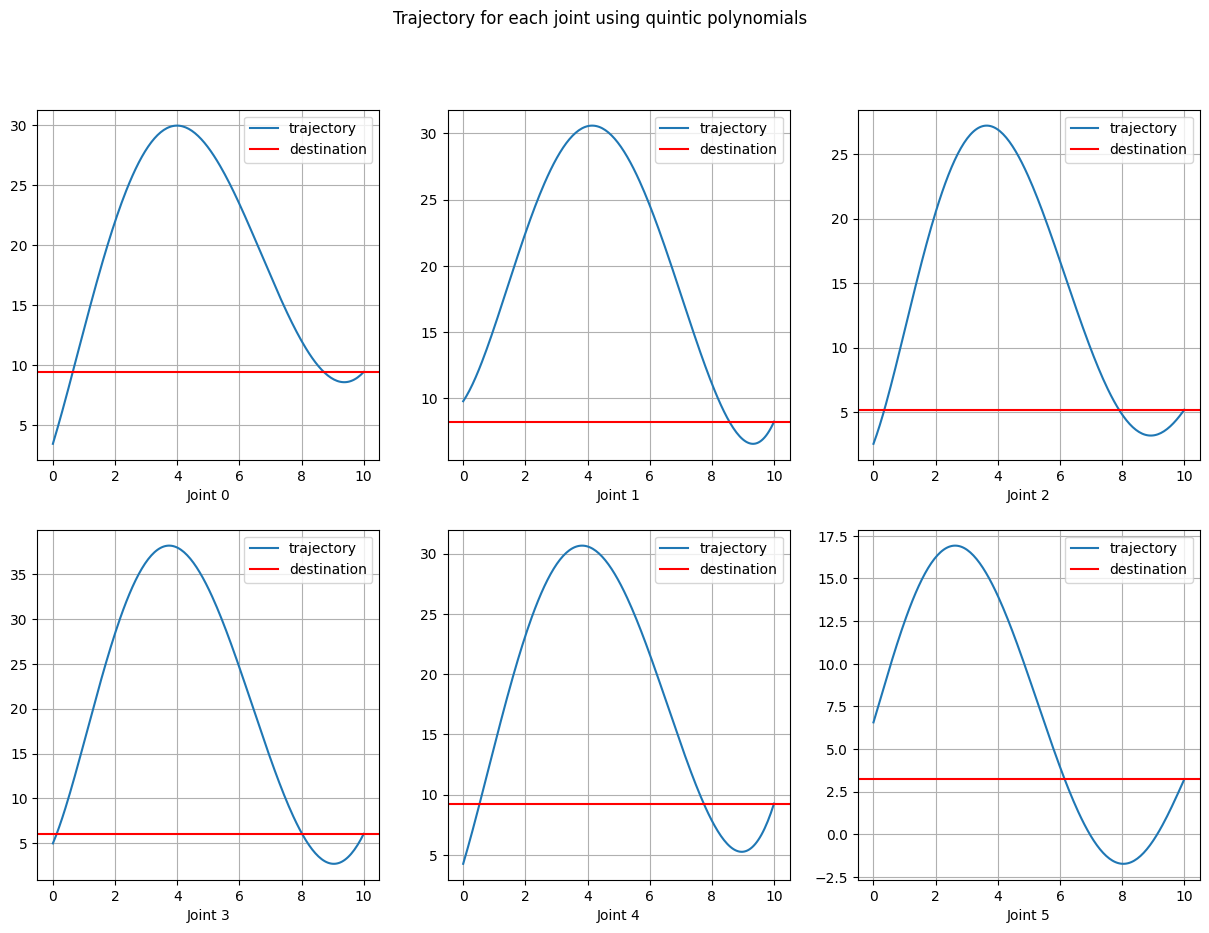
\includegraphics[width=\linewidth]{images/trajectory_polynomial.png}